%!TEX root = ../main.tex

\section{Supplementary Experimental Results}
\label{sec:appendix_experiments}

In this section, we provide supplementary experimental results, including sensitivity analyses, time and memory usage, data size bucket details, pipeline length and table number analyses, error analysis on real-world data, model size scaling results, and training hyperparameters.

\subsection{Sensitivity Analysis: Exploration Turns}
\label{subsec:appendix_sensitivity_turns}

\begin{figure}[t]
    \centering
    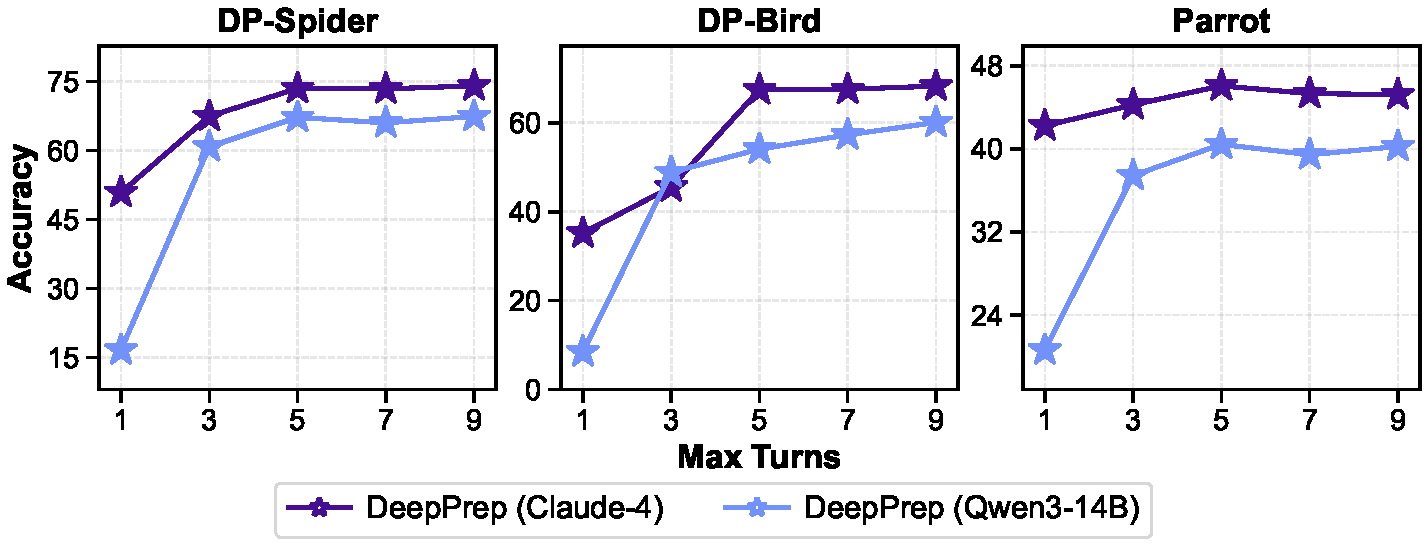
\includegraphics[width=1.01\columnwidth]{plots/plot/performance_vary_maxturn_accuracy.pdf}
    \vspace{-2em} 
    \caption{Accuracy of \sys when changing the maximum number of exploration turns.}
    \label{\labelprefix fig:performance_vary_maxturn_accuracy}
    \vspace{-1em}
\end{figure}

\begin{figure}[t]
    \centering
    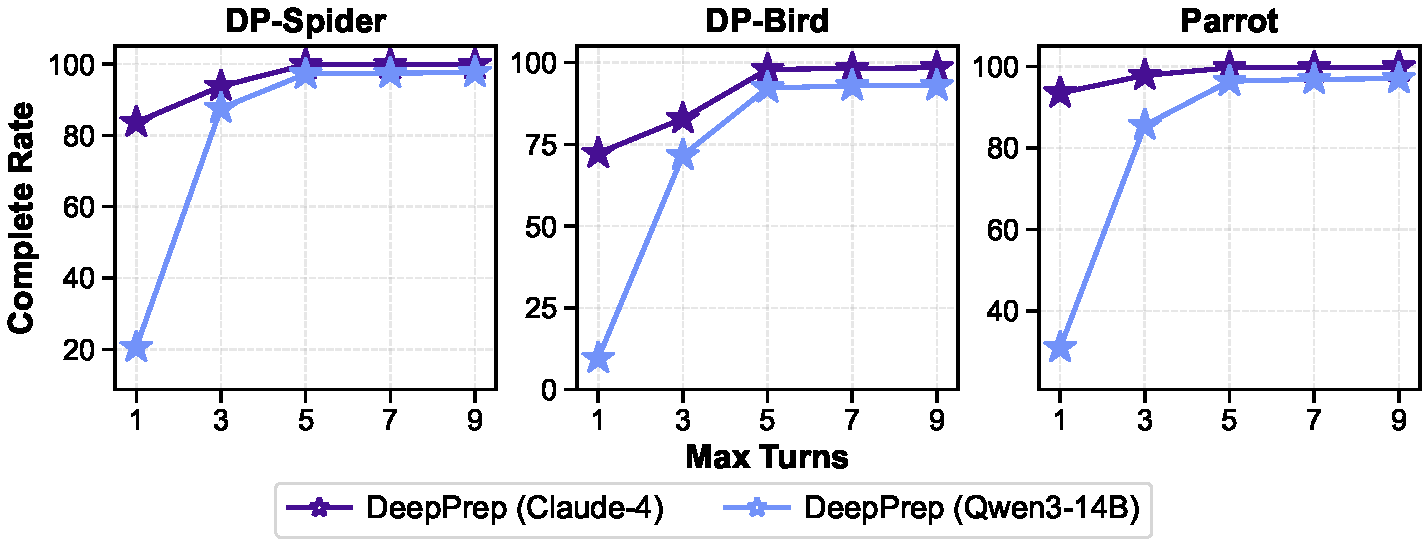
\includegraphics[width=1.01\columnwidth]{plots/plot/performance_vary_maxturn_complete_rate.pdf}
    \vspace{-2em} 
    \caption{Completion rate of \sys when changing the maximum number of exploration turns.}
    \label{\labelprefix fig:performance_vary_maxturn_complete_rate}
    \vspace{-1em}
\end{figure}

Figure~\ref{\labelprefix fig:performance_vary_maxturn_accuracy} and Figure~\ref{\labelprefix fig:performance_vary_maxturn_complete_rate} show the impact of the maximum number of exploration turns on accuracy and completion rate, respectively. Overall, the performance of \sys improves as the exploration turn increases and stabilizes at around five turns across all datasets and model backbones. For example, on Claude-4, increasing the budget from one to five turns improves accuracy by 22.63 points on Synth-Spider and 32.21 points on Synth-Bird. Beyond five turns, the additional gain is less than one point. This indicates that \sys can solve most ADP cases within five exploration turns. As illustrated in Figure~\ref{\labelprefix fig:performance_vary_maxturn_complete_rate}, \sys successfully completes the ADP task at nearly 100\% completion rate with five turns.

\subsection{Sensitivity Analysis: Data Size}
\label{subsec:appendix_sensitivity_data_size}

\begin{figure}[t]
    \centering
    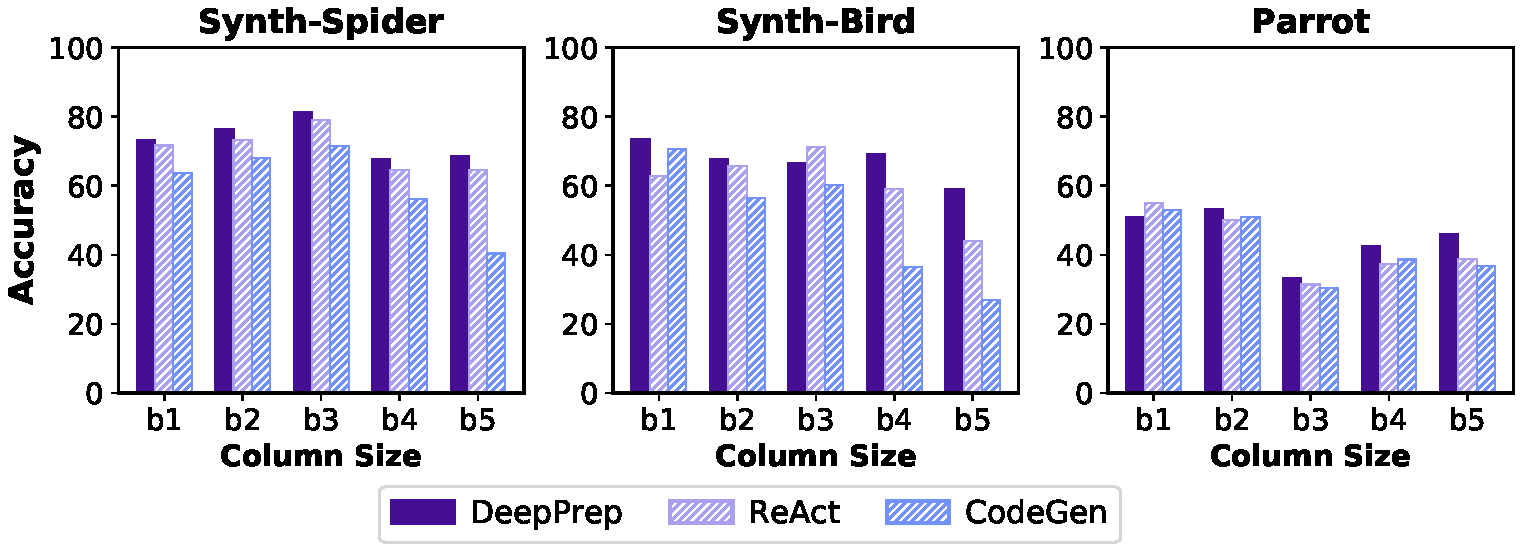
\includegraphics[width=1.01\columnwidth]{plots/plot/performance_compare_by_column_size_acc.pdf}
    \vspace{-2em} 
    \caption{Accuracy comparison on tables with varying number of columns. For Synth-Spider, b1 (1-4), b2 (5-7), b3 (8-9), b4 (10-14), b5 (15-124,843). For Synth-Bird, b1 (1-11), b2 (12-27), b3 (29-74), b4 (75-1,003), b5 (1,004-20,015). For Parrot, b1 (2-4), b2 (5-7), b3 (8-11), b4 (12-16), b5 (18-587).}
    \label{\labelprefix fig:performance_compare_by_column_size_acc}
    \vspace{-1em}
\end{figure}

\begin{figure}[t]
    \centering
    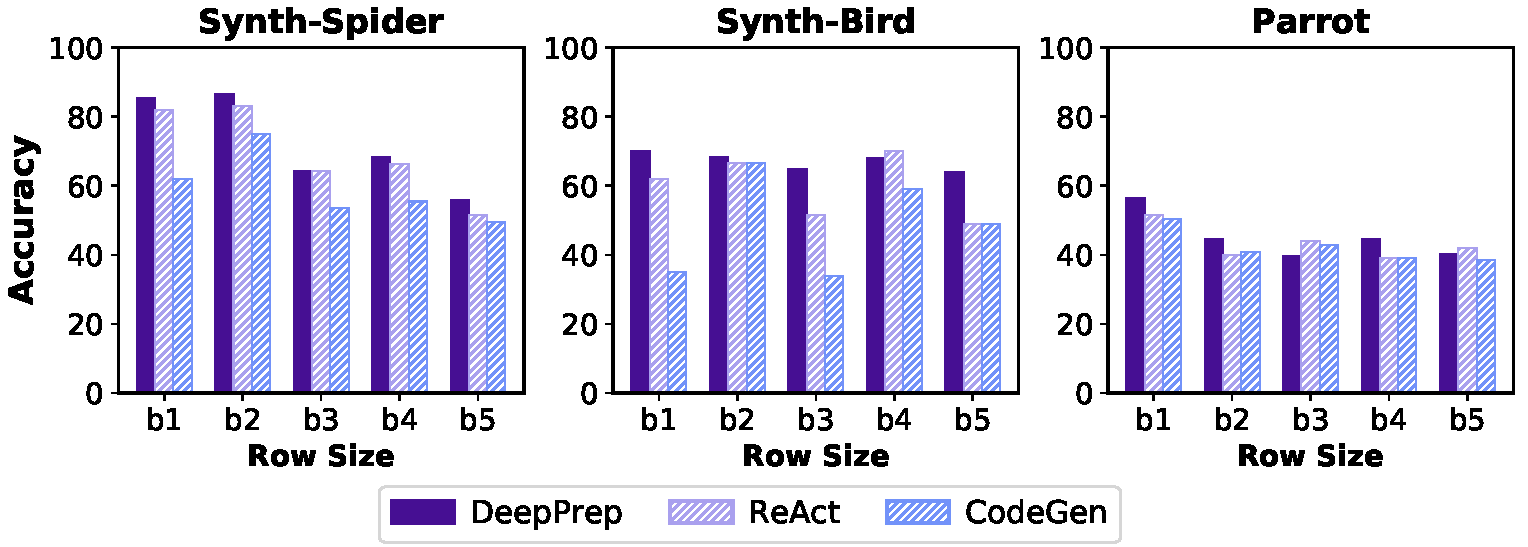
\includegraphics[width=1.01\columnwidth]{plots/plot/performance_compare_by_row_size_acc.pdf}
    \vspace{-2em} 
    \caption{Accuracy comparison on tables with varying number of rows. For Synth-Spider, b1 (1-9), b2 (10-15), b3 (16-21), b4 (22-35), b5 (36-124,842). For Synth-Bird, b1 (1-110), b2 (115-1,000), b3 (1,001-1,022), b4 (1,023-2,004), b5 (2,005-360,006). For Parrot, b1 (2-13), b2 (14-30), b3 (31-100), b4 (107-2,000), b5 (2,075-200,000).}
    \label{\labelprefix fig:performance_compare_by_row_size_acc}
    \vspace{-1em}
\end{figure}


Figures~\ref{\labelprefix fig:performance_compare_by_column_size_acc} and~\ref{\labelprefix fig:performance_compare_by_row_size_acc} show the accuracy of \sys and baselines under varying column sizes and row sizes, respectively. \sys remains robust on small and medium-sized tables. Performance degrades only for the largest buckets, where the table sampling strategy may omit relevant information from the sampled content for very large tables.

\subsection{Time and Memory Usage}
\label{subsec:appendix_time_memory}

\begin{table}[t]
  \centering
  \caption{\bf Average Execution Time (s) and Memory Usage (MB) under Varying Data and Task Complexity.}
  \vspace{-1em}
  \label{\labelprefix tbl:avg_time_memory_by_data_characteristics}
  \resizebox{0.99\columnwidth}{!}{
    \begin{tabular}{|c|c||c|c|c|c|c|c|}
      \hline
      \multirow{2}{*}{\textbf{Data Type}} 
      & \multirow{2}{*}{\textbf{Group}}
      & \multicolumn{2}{c|}{\textbf{Synth-Spider}}
      & \multicolumn{2}{c|}{\textbf{Synth-Bird}}
      & \multicolumn{2}{c|}{\textbf{Parrot}} \\
      \cline{3-8}
      & 
      & \textbf{Time} & \textbf{Mem.}
      & \textbf{Time} & \textbf{Mem.}
      & \textbf{Time} & \textbf{Mem.} \\
      \hline \hline

      \multirow{5}{*}{\shortstack{\textbf{Column}\\\textbf{Size}}}
      & b1
      & 8.91 & 66.31
      & 11.46 & 77.34
      & 7.09 & 114.42 \\
      \cline{2-8}

      & b2
      & 8.21 & 66.54
      & 12.13 & 74.07
      & 9.76 & 116.51 \\
      \cline{2-8}

      & b3
      & 8.48 & 67.07
      & 12.12 & 85.35
      & 11.49 & 125.12 \\
      \cline{2-8}

      & b4
      & 10.19 & 69.32
      & 12.88 & 83.31
      & 10.36 & 137.34 \\
      \cline{2-8}

      & b5
      & 11.30 & 68.37
      & 13.78 & 90.70
      & 11.36 & 143.35 \\
      \hline
      \hline

      \multirow{5}{*}{\shortstack{\textbf{Row}\\\textbf{Size}}}
      & b1
      & 7.87 & 65.69
      & 11.48 & 88.66
      & 9.54 & 124.43 \\
      \cline{2-8}

      & b2
      & 8.13 & 65.99
      & 11.36 & 74.92
      & 10.57 & 124.72 \\
      \cline{2-8}

      & b3
      & 9.30 & 66.78
      & 13.57 & 79.24
      & 9.07 & 120.89 \\
      \cline{2-8}

      & b4
      & 10.63 & 68.33
      & 12.64 & 80.00
      & 10.13 & 127.47 \\
      \cline{2-8}

      & b5
      & 11.72 & 71.30
      & 13.96 & 88.31
      & 10.77 & 135.00 \\
      \hline
      \hline

      \multirow{3}{*}{\shortstack{\textbf{Operator}\\\textbf{Length}}}
      & g1
      & 8.54 & 66.74
      & 11.26 & 80.08
      & 6.85 & 114.01 \\
      \cline{2-8}

      & g2
      & 12.75 & 70.30
      & 14.58 & 85.02
      & 11.06 & 130.69 \\
      \cline{2-8}

      & g3
      & 14.62 & 68.53
      & 14.01 & 81.92
      & 12.22 & 132.31 \\
      \hline
      \hline

      \multirow{3}{*}{\shortstack{\textbf{Table}\\\textbf{Number}}}
      & 1
      & 8.06 & 66.51
      & 9.94 & 79.00
      & 9.58 & 124.41 \\
      \cline{2-8}

      & 2
      & 10.54 & 68.82
      & 13.11 & 83.38
      & 10.81 & 128.74 \\
      \cline{2-8}

      & $\geq$3
      & 13.49 & 68.54
      & 14.92 & 81.08
      & -- & -- \\
      \hline
    \end{tabular}
  }
  \vspace{-1em}
\end{table}


Table~\ref{\labelprefix tbl:avg_time_memory_by_data_characteristics} reports the average execution time and memory usage across different data and task complexity groups. \sys exhibits stable growth in both execution time and memory usage as workload complexity increases. For example, on Synth-Spider, the average execution time increases only from 8.91 to 11.30 seconds when moving from the smallest to the largest column-size bucket, while memory usage remains between 66 MB and 69 MB. Similar trends are observed on Synth-Bird and Parrot. These results indicate that \sys scales gracefully with increasing data size and task complexity.

\stitle{Why \sys Scales Stably.}
The stable scaling behavior can be explained by the generative search framework formalized in Algorithm~\ref{alg:sys}. At each step, the agent generates a \action{plan} $\psi_t$ (Line 3) and an \action{expand} action (Line 4), followed by the execution of the proposed operators (Line 7). The process is bounded by the maximum exploration turn $T$ and the maximum operator sequence length $L$ per expansion, yielding a worst-case complexity of $O(T \times L)$. Unlike classical tree-search methods such as MCTS, which explicitly expand and evaluate many candidate branches, \sys generates only one operator pipeline conditioned on the current tree state. The ``pruning'' is implicit in the LLM's decision-making: the agent observes failure traces and avoids revisiting failed branches, rather than enumerating all possible expansions. Consequently, the effective branching factor depends on the LLM's learned policy and remains bounded regardless of input size, which explains the stable growth in time and memory usage.

\subsection{Data Size Bucket Details}
\label{subsec:appendix_bucket_details}

For row-size and column-size analyses, we sort all cases by the corresponding metric and divide them into five equal-width buckets $b_1 - b_5$, as described below.

\begin{itemize}[leftmargin=*]
    \item \textbf{The Synth-Spider dataset.}
    \begin{itemize}
        \item Column buckets: $b_1$ (1--4), $b_2$ (5--7), $b_3$ (8--9), $b_4$ (10--14), $b_5$ (15--124,843).
        \item Row buckets: $b_1$ (1--9), $b_2$ (10--15), $b_3$ (16--21), $b_4$ (22--35), $b_5$ (36--124,842).
    \end{itemize}
    \item \textbf{The Synth-Bird dataset.}
    \begin{itemize}
        \item Column buckets: $b_1$ (1--11), $b_2$ (12--27), $b_3$ (29--74), $b_4$ (75--1,003), $b_5$ (1,004--20,015).
        \item Row buckets: $b_1$ (1--110), $b_2$ (115--1,000), $b_3$ (1,001--1,022), $b_4$ (1,023--2,004), $b_5$ (2,005--360,006).
    \end{itemize}
    \item \textbf{The Parrot dataset.}
    \begin{itemize}
        \item Column buckets: $b_1$ (2--4), $b_2$ (5--7), $b_3$ (8--11), $b_4$ (12--16), $b_5$ (18--587).
        \item Row buckets: $b_1$ (2--13), $b_2$ (14--30), $b_3$ (31--100), $b_4$ (107--2,000), $b_5$ (2,075--200,000).
    \end{itemize}
\end{itemize}

\subsection{Pipeline Length and Table Number Analysis}
\label{subsec:appendix_pipeline_table}

\begin{figure}[t]
    \centering
    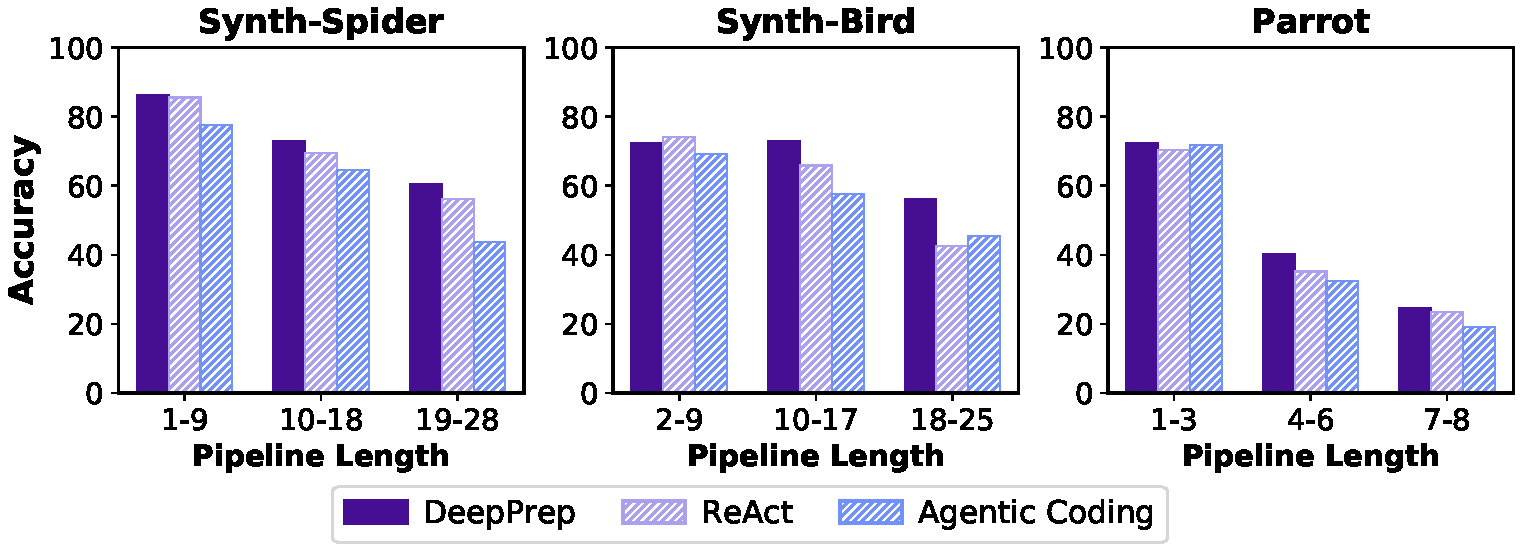
\includegraphics[width=1.01\columnwidth]{plots/plot/performance_compare_on_task_diff_claude.pdf}
    \vspace{-2em} 
    \caption{Comparison on Accuracy with varying Pipeline Length.}
    \label{\labelprefix fig:performance_compare_on_task_diff_claude}
    \vspace{-1em}
\end{figure}

\begin{figure}[t]
    \centering
    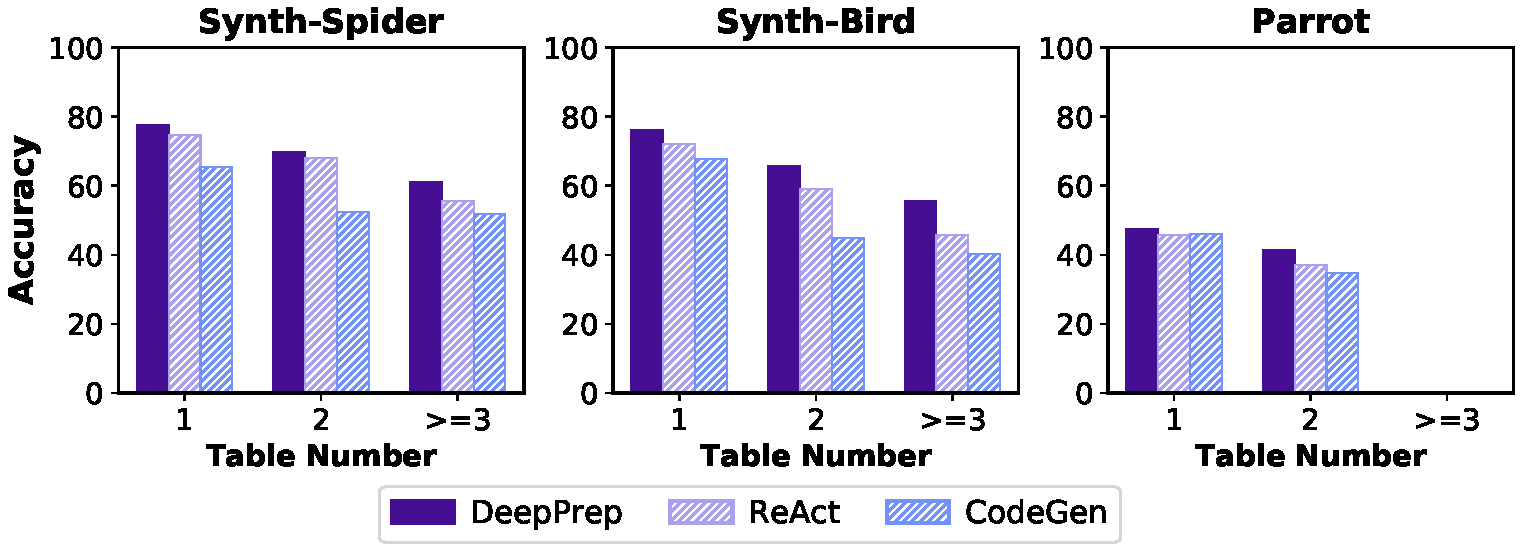
\includegraphics[width=1.01\columnwidth]{plots/plot/performance_compare_by_table_number_acc.pdf}
    \vspace{-2em} 
    \caption{Comparison on Accuracy with varying number of source tables.}
    \label{\labelprefix fig:performance_compare_by_table_number_acc}
    \vspace{-0.5em}
\end{figure}


\stitle{Pipeline Length.}
For pipeline length, we partition ADP cases into Simple, Medium, and Complex groups according to the number of operators in the target pipeline. As shown in Figure~\ref{\labelprefix fig:performance_compare_on_task_diff_claude}, all methods degrade as the pipeline length increases. However, \sys shows the smallest degradation, and its advantage over baselines becomes larger on Complex cases. On Synth-Spider, \sys achieves 60.5 accuracy on Complex cases, outperforming CodeGen by 16.8 points.

\stitle{Table Number.}
As shown in Figure~\ref{\labelprefix fig:performance_compare_by_table_number_acc}, performance generally decreases as more source tables are involved, but \sys consistently achieves the highest accuracy across different table number groups.

\subsection{Error Analysis on Real-World Dataset}
\label{subsec:appendix_error_analysis}

\begin{figure}[t]
    \centering
    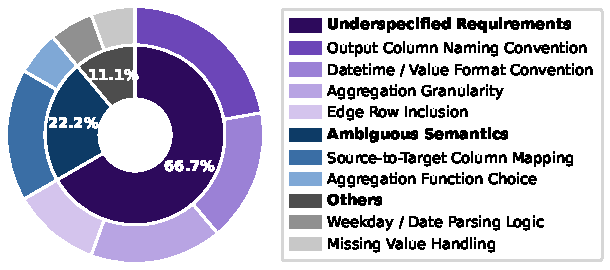
\includegraphics[width=1.01\columnwidth]{plots/plot/error_analysis_pie.pdf}
    \vspace{-2em} 
    \caption{Error analysis on Buildings.}
    \label{\labelprefix fig:error_analysis_pie}
    \vspace{-1em}
\end{figure}

Figure~\ref{\labelprefix fig:error_analysis_pie} presents the error analysis of \sys on the Buildings dataset. The analysis reveals three major sources of errors:

\begin{itemize}[leftmargin=*]
    \item \textbf{Ambiguous column semantics} (50\% of failures): Real cases often contain abbreviated or domain-specific column names (\eg \texttt{hdd}, \texttt{cdd}), which lead to selecting the wrong columns required to be mapped or aggregated into the target columns.
    \item \textbf{Underspecified requirements} (33\% of failures): In real-world scenarios, the target specification is often described only at a high level, without explicitly defining important details such as the desired aggregation granularity (\eg daily versus monthly). This increases the reasoning burden of the model during the data preparation stage.
    \item \textbf{Domain logic errors} (11\% of failures): Some failures are caused by incorrect domain-specific logic, such as applying the wrong aggregation function or misinterpreting the semantic relationship between columns.
\end{itemize}

These findings not only provide additional evidence that Buildings captures realistic ADP challenges, but also highlight important directions for future work.

\subsection{Model Size Scaling Results}
\label{subsec:appendix_model_scaling}

\begin{figure}[t]
    \centering
    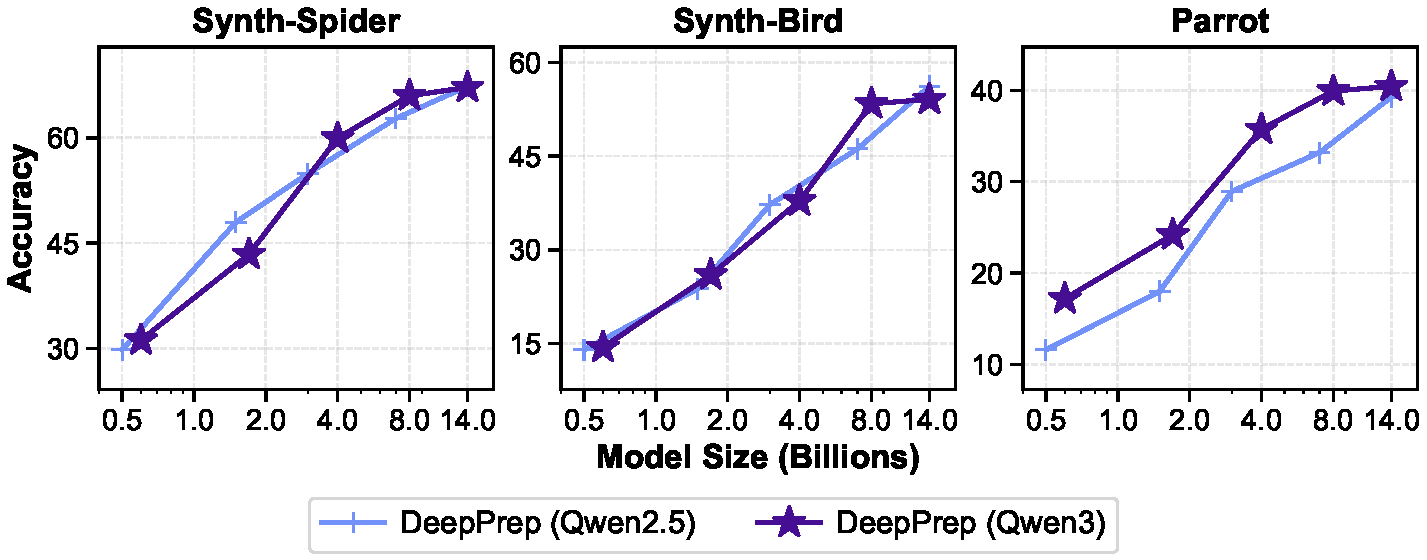
\includegraphics[width=1.01\columnwidth]{plots/plot/performance_scale_accuracy_only.pdf}
    \vspace{-1.5em} 
    \caption{Performance scales with larger model size.
    % \fmh{Results of Qwen2.5 are not updated (Use 2025 version).} 
    }
    \label{\labelprefix fig:performance_scale_accuracy_only}
    \vspace{-0.5em} 
  %\vspace{-1em}
\end{figure}

Figure~\ref{\labelprefix fig:performance_scale_accuracy_only} shows the performance of \sys with backbone models of varying sizes across the Qwen2.5 and Qwen3 families. Accuracy steadily increases with model size. On Synth-Spider, scaling Qwen3 from 0.6B to 14B improves accuracy from 31.20 to 67.18. Across comparable model sizes, the Qwen3 series also shows stronger out-of-domain performance than Qwen2.5. For example, on Synth-Bird, Qwen3-8B achieves 53.39 accuracy versus 46.17 for Qwen2.5-7B. These results suggest \sys benefits from stronger backbone models and maintains positive scaling trends.

\subsection{Training Hyperparameters}
\label{subsec:appendix_training_params}

\begin{table}[t]
    \centering
    \caption{\bf Detailed experimental settings.}
    \vspace{-1em}
    \label{tbl:appendix_hyperparameters}
    
    % --- Subtable 1: Operator Learning ---
    \begin{subtable}[t]{\columnwidth}
        \centering
        \caption{\bf{Hyperparameters for Operator Learning.}}
        \label{subtbl:hyper_op_learning}
        \vspace{-0.15em}
        \resizebox{0.5\linewidth}{!}{
        \begin{tabular}{|l||c|}
            \hline
            \textbf{Hyperparameter} & \textbf{Value} \\
            \hline \hline
            Base Model & Qwen3-8B \\
            Global Batch Size & 256 \\
            Learning Rate & 1e-5 \\
            Epochs & 3 \\
            Max Sequence Length & 16,384 \\
            Warmup Ratio & 0.05 \\
            Precision & bfloat16 \\
            \hline
        \end{tabular}
        }
    \end{subtable}
    
    \vspace{0.30em}
    
    % --- Subtable 2: Cold Start SFT ---
    \begin{subtable}[t]{\columnwidth}
        \centering
        \caption{\bf{Hyperparameters for Tree-based Agentic Reasoning SFT.}}
        \label{subtbl:hyper_cold_start}
        \vspace{-0.15em}
        \resizebox{0.5\linewidth}{!}{
        \begin{tabular}{|l||c|}
            \hline
            \textbf{Hyperparameter} & \textbf{Value} \\
            \hline \hline
            Base Model & Stage 1 Ckp \\
            Global Batch Size & 256 \\
            Learning Rate & 6e-5 \\
            Epochs & 15 \\
            Max Sequence Length & 24,000 \\
            Warmup Ratio & 0.05 \\
            Precision & bfloat16 \\
            \hline
        \end{tabular}
        }
    \end{subtable}
    
    \vspace{0.30em}
    
    % --- Subtable 3: RL ---
    \begin{subtable}[t]{\columnwidth}
        \centering
        \caption{\bf{Hyperparameters for Multi-Turn RL.}}
        \label{subtbl:hyper_rl}
        \vspace{-0.15em}
        \resizebox{0.5\linewidth}{!}{
        \begin{tabular}{|l||c|}
            \hline
            \textbf{Hyperparameter} & \textbf{Value} \\
            \hline \hline
            Algorithm & GRPO \\
            Global Batch Size & 64 \\
            Learning Rate & 1e-6 \\
            Epochs & 1 \\
            Group Size ($G$) & 8 \\
            KL Coefficient ($\beta$) & 0.005 \\
            Temperature / Top-p & 0.6 / 0.95 \\
            Max Total Length & 28,000 \\ 
            Max Response Length & 2000 \\
            Max Exploration Turn & 5 \\
            Max Prompt Length & 12000 \\
            \hline
        \end{tabular}
        }
    \end{subtable}
    
\end{table}


Table~\ref{tbl:appendix_hyperparameters} summarizes the specific hyperparameters for each training stage of \sys.

\stitle{Stage 1: Operator Syntax Learning.}
As defined in Section~\ref{subsec:cold_start}, the goal of this stage is to focus on the syntax and semantics of individual operators. We set the learning rate to 1e-5 with a cosine scheduler and a warmup ratio of 0.05. Since this stage mainly involves generating short operator sequences, we set the maximum sequence length to 16,384. We train the model for 3 epochs with a global batch size of 256.

\stitle{Stage 2: Reasoning Procedure Learning.}
This stage corresponds to aligning the model with the tree-based agentic reasoning mechanism in Section~\ref{subsec:cold_start}. We initialize the model using the checkpoint from Stage 1. The objective is to teach the model to perform global planning, exploration, and backtracking using the agentic reasoning tree. To accommodate the large context of the agentic reasoning tree and multi-turn interaction history, we increase the maximum sequence length to 24,000. We use a learning rate of 6e-5 to effectively learn the complex reasoning patterns. The training runs for 15 epochs with a global batch size of 256.

\stitle{Stage 3: Multi-turn RL with Hybrid Reward.}
In the final stage, we apply the multi-turn RL with hybrid reward described in Section~\ref{subsec:rl_reward}. We utilize the Group Relative Policy Optimization (GRPO) algorithm to optimize the model's decision-making strategy. During training, we sample $G=8$ trajectories for each prompt to estimate the baseline. We use a small learning rate of 1e-6 and set the KL divergence coefficient ($\beta$) to 0.005 to ensure training stability. To handle long-horizon tasks, we set the maximum total length to 28,000 and the maximum prompt length to 12,000. We limit the maximum exploration turns to 5 and the response length for each step to 2,000 tokens.

\stitle{Training Data.}
Due to time and computational constraints, we utilized a curated subset of the synthesized data for training rather than the full dataset. For the initial stage, we constructed a dataset of 8,000 samples. These samples focus on basic operator usage to establish the model's fundamental understanding of the operator space. In the SFT stage, we employed five open-source LLMs as teacher models to generate diverse reasoning trajectories. We initially distilled approximately 20,000 trajectories. To ensure high training quality, we filtered these trajectories based on the process reward function $R_{\text{llm}}$ score (retaining scores $> 0.8$) and the number of interaction turns. This process yielded a final dataset of 11,198 high-quality samples. For the reinforcement learning stage, we randomly sampled 4,000 instances from the Synth-Spider dataset.

\subsection{Model Size Scaling Study}
\label{subsec:appendix_model_size_scale}

\begin{figure}[t]
    \centering
    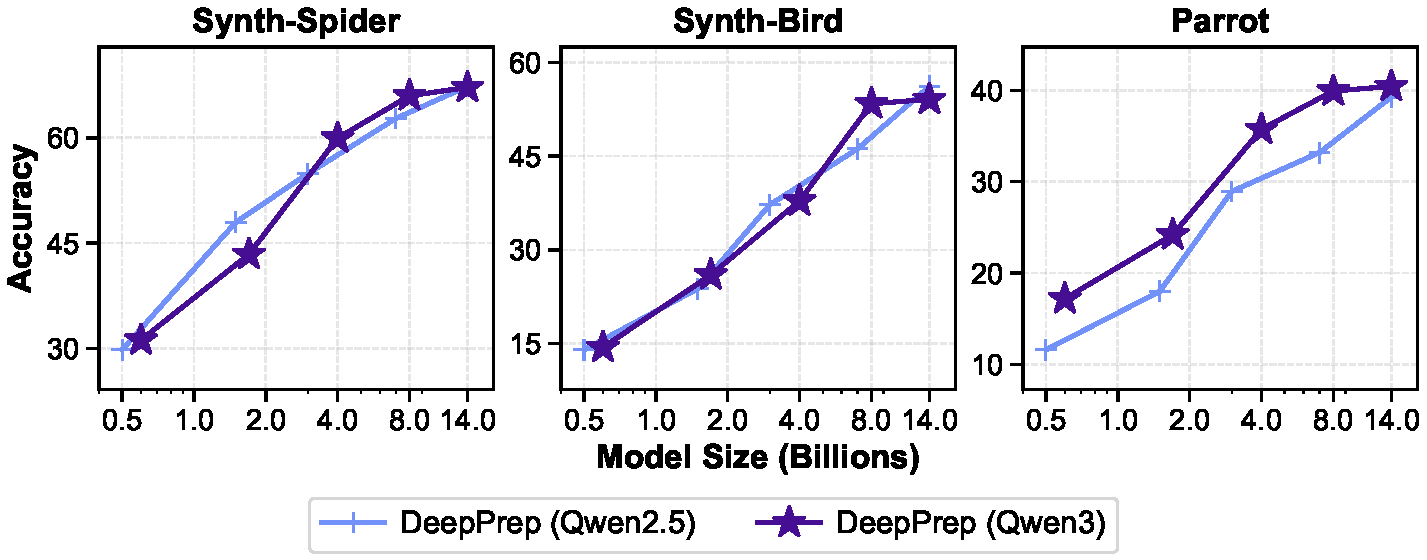
\includegraphics[width=1.01\columnwidth]{plots/plot/performance_scale_accuracy_only.pdf}
    \vspace{-1.5em} 
    \caption{Performance scales with larger model size.
    % \fmh{Results of Qwen2.5 are not updated (Use 2025 version).} 
    }
    \label{\labelprefix fig:performance_scale_accuracy_only}
    \vspace{-0.5em} 
  %\vspace{-1em}
\end{figure}

\stitle{Exp-\expnum\label{exp:model_scaling}: Model Size Scaling Study.}
We study how \sys performs under different backbone model sizes. We train \sys with LLM backbones ranging from 0.5B to 14B parameters across the Qwen2.5 and Qwen3 families.
Figure~\ref{\labelprefix fig:performance_scale_accuracy_only} shows that accuracy steadily increases with model size. On Synth-Spider, scaling Qwen3 from 0.6B to 14B improves Accuracy from 31.20 to 67.18. Across comparable model sizes, the Qwen3 series also shows stronger out-of-domain performance than Qwen2.5. For example, on Synth-Bird, Qwen3-8B achieves 53.39 Accuracy versus 46.17 for Qwen2.5-7B. These results suggest \sys benefits from stronger backbone models and maintains positive scaling trends.

\begin{shaded}
\noindent
\textbf{Finding \findingnum: The performance of \sys improves with larger backbone model sizes, which suggest that \sys benefits from stronger backbone models and maintains positive scaling trends.}
\end{shaded}
